% Figura cuerpo B2 (3.1): las tres piezas del argumento y lo que aporta cada una.
\documentclass[tikz,border=3pt]{standalone}
\usepackage[T1]{fontenc}
\usepackage[utf8]{inputenc}
\usepackage{amsmath}
\usetikzlibrary{arrows.meta,calc,positioning}
\begin{document}
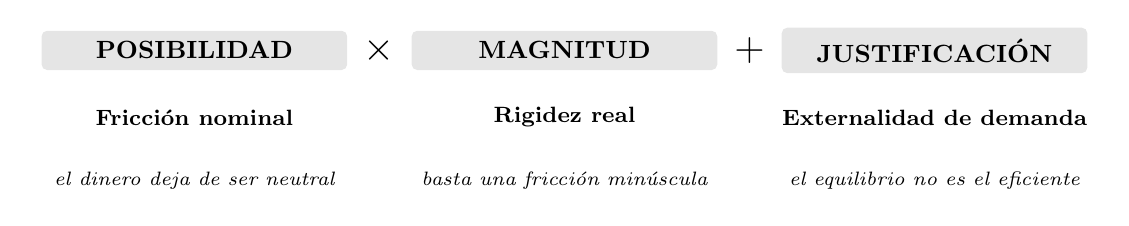
\begin{tikzpicture}[font=\scriptsize,
  clave/.style={fill=black!10, rounded corners=2pt, align=center, inner sep=4pt,
                text width=3.6cm, font=\small\bfseries},
  pieza/.style={align=center, text width=3.9cm, font=\footnotesize\bfseries},
  glosa/.style={align=center, text width=4.0cm, font=\scriptsize\itshape},
  op/.style={font=\Large}]

  \def\cx{4.7}
  \node[clave] (k1) at (0,1.30)      {POSIBILIDAD};
  \node[clave] (k2) at (\cx,1.30)    {MAGNITUD};
  \node[clave] (k3) at (2*\cx,1.30)  {JUSTIFICACIÓN};

  \node[pieza] (c1) at (0,0.45)      {Fricción nominal};
  \node[pieza] (c2) at (\cx,0.45)    {Rigidez real};
  \node[pieza] (c3) at (2*\cx,0.45)  {Externalidad de demanda};

  \node[glosa] (g1) at (0,-0.35)     {el dinero deja de ser neutral};
  \node[glosa] (g2) at (\cx,-0.35)   {basta una fricción minúscula};
  \node[glosa] (g3) at (2*\cx,-0.35) {el equilibrio no es el eficiente};

  \node[op] at ({\cx/2},1.30)   {$\times$};
  \node[op] at ({3*\cx/2},1.30) {$+$};
\end{tikzpicture}
\end{document}
